\documentclass{article}
\pdfpagewidth=8.5in
\pdfpageheight=11in
% \usepackage{ijcai19}
%\usepackage[utf8]{inputenc}
\usepackage{graphicx}
\usepackage{array}
\usepackage{changepage}
\usepackage{float}
\usepackage{tabu}
\usepackage{longtable}
\usepackage{multirow}

\title{Supplementary Material: Exploring Computational User Models for Agent Policy Summarization}
\date{}

\author{
Isaac Lage, 
Daphna Lifschitz,
Finale Doshi-Velez,
Ofra Amir
}

\begin{document}
\maketitle

\section{Computational Experiment Details}

\paragraph{State Representations.} 
In the PAC-MAN and random gridworld domains, we used different feature sets for IL and IRL so that IL would have access to some short-term temporal information. In PAC-MAN, we use distance to nearest food, an indicator for food consumption, and an indicator for being eaten by a ghost as features for the IRL model, and the direction of nearest food, an indicator for collisions with ghosts or walls in each direction for the IL model. In the random gridworld, we used the 5-dimensional vector as features for the IRL model, and we additionally used the concatenated vector for each neighboring tile for the IL model. In the HIV simulator domain, we used the 6 biomarkers as features for both IL and IRL. 

The continuous HIV simulator domain, required discretization to build the explicit transition function required by the IRL model. To do this, we ran K-Means clustering with 100 clusters on each state in the extracted trajectories, and used the cluster centers as the state representations.\footnote{100 clusters resulted in accuracy above $0.95$ when using the most common action in each cluster for prediction.} We use this representation for the IRL reconstruction and to compute the value, but otherwise we use the original state representations.

\paragraph{Fixed Max-Ent Hyperparameters}

We held the following choices for the IRL model fixed. We set the discount factor to $\gamma = 0.95$ for Random Gridworld, $\gamma = 0.98$ for HIV to match the discount factor used to derive the policy.  For PAC-MAN, the policy was derived without a discount factor so we set it to $\gamma = 0.95$. In the Random Gridworld and PAC-MAN domains, we set the rollout horizon to 10, while in the longer time-horizon HIV domain we set the rollout horizon to 25. For Max-Ent, we set the learning rate to 1 for the random gridworld, 0.1 for PAC-MAN and 0.01 for the HIV simulator and ran 100 iterations, stopping if the rewards changed by less than 1e-5 between two consecutive iterations.

\section{Hyperparameters}

\begin{figure}[h]
\centering
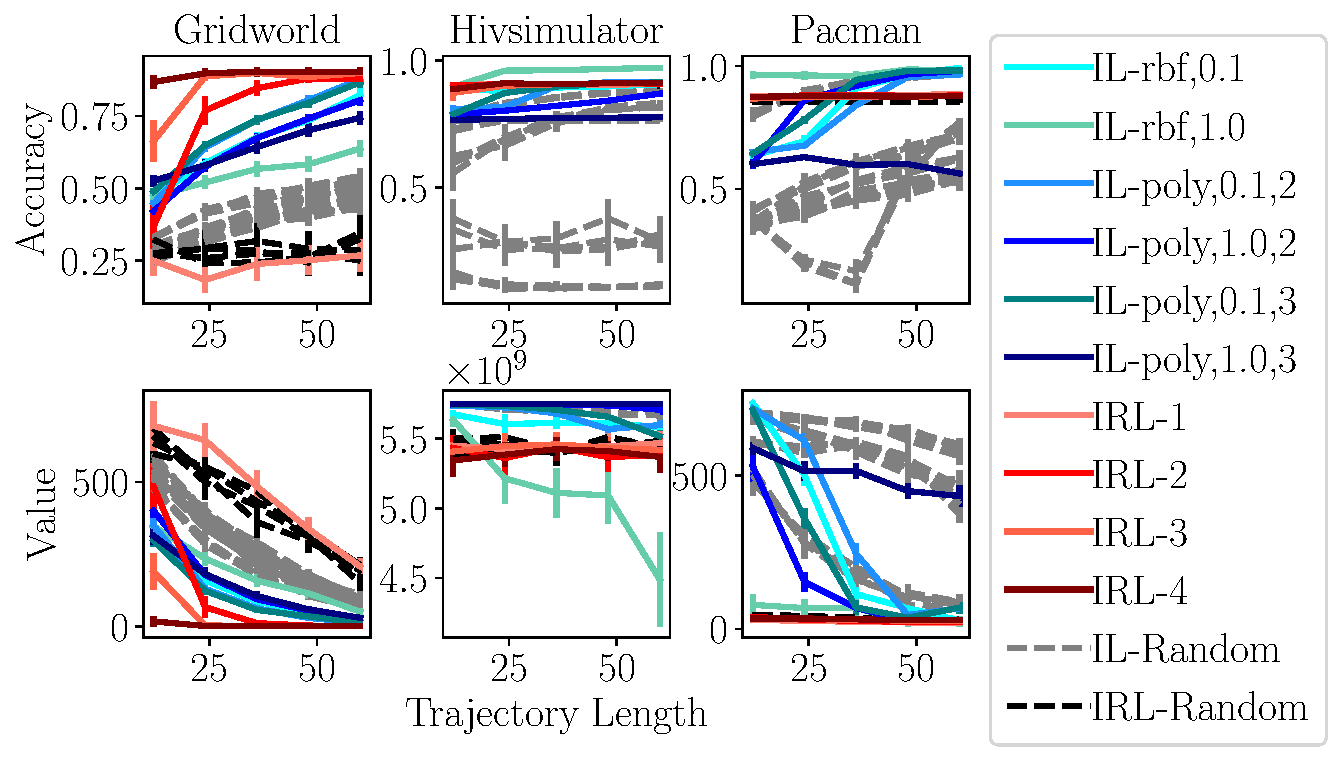
\includegraphics[width=1\columnwidth]{figures/reconstruction_by_summary_size_hyperparams.pdf}
\caption{Reconstruction accuracy across a variety of reconstruction methods and hyper-parameter settings (assuming the same extraction method), by summary size, averaged over 75 random restarts. Error bars signify 95\% confidence intervals. We chose the smallest summary size such that increasing it does not result in changes in the best performing methods for either IL or IRL in the HIV simulator and PAC-MAN domains where this was possible. In the random gridworld domain, increasing the summary size always improved the performance of the IL methods, so we choose a summary size such that the best performing IRL methods did not change (HIV: 24; Gridworld: 24; PAC-MAN: 12).}
\label{fig:hyperparameters}
\end{figure}

We chose summary sizes and hyperparameter settings to analyze reconstruction quality by plotting the reconstruction quality of each hyperparameter setting for IL and IRL with the summary extracted using the corresponding model. Figure~\ref{fig:hyperparameters} shows this for 75 random restarts over summary sizes [12, 24, 36, 48, 60]; IL hyperparameters: kernel [RBF, polynomial], length scale [0.1, 1.] and degree [2, 3] (for polynomial kernel only); and IRL hyperparameters: trajectory lengths [1, 2, 3, 4]. The error bars correspond to 95\% confidence intervals.

For each reconstruction method, we additionally plotted the reconstruction quality with a random summary. For IL, we used only random summaries with trajectory length [1], and for the IRL, we tried random summaries with trajectory lengths [1, 2, 3, 4].

To determine the summary size $k$ for each domain, we chose the smallest summary size such that increasing it does not result in changes in the best performing methods for either IL or IRL in the HIV simulator and PAC-MAN domains where this was possible. In the random gridworld domain, increasing the summary size always improved the performance of the IL methods, so we choose a summary size such that the best performing IRL methods did not change (HIV: 24; Gridworld: 24; PAC-MAN: 12).  Our results in the main paper show only the best performing methods for IL and IRL at that summary size.

%Ike: Should we include an analysis of this figure? Or only how it figures in our main results?

\section{User Study Summaries}

We selected a single summary for each model in each domain, and a single set of 9 test questions for each domain in order to run the human-subject studies. We chose summaries and test states to have a similar pattern of high-accuracy reconstructions when the summarization model matches the extraction model, and low-accuracy reconstructions when the reconstruction model and the extraction model do not match. The summaries and test states we chose resulted in the reconstruction accuracies listed in Table~\ref{tab:gridworld_summaries}. 

The absolute values of the HIV summaries are different than those listed in Figure 1 of the main text because we used a shorter summary (12 states instead of 24) so that it could be easily visualized on a single page of the experiment. The accuracies computed on only the test states do not perfectly match the accuracies of the entire test grid, but they do preserve the pattern mentioned above of higher accuracies when reconstruction model and extraction model match, and lower otherwise. This allows us to test whether people's reconstructions have a difference in quality with different summaries.

\begin{table}[]
\centering
\begin{tabular}{ll|ll|ll}
\multicolumn{2}{c}{ } &            \multicolumn{2}{c}{HIV}  &  \multicolumn{2}{c}{Gridworld}  \\
            &               & IL   & IRL  &   IL   & IRL  \\ \hline 
\multirow{ 2}{*}{All States}  & IL            & 0.89 & 0.44 &  0.63 & 0.20 \\
            & IRL           & 0.76 & 0.91 & 0.24 & 0.91 \\ \hline 
\multirow{ 2}{*}{Test States} & IL            & 0.67 & 0.33 & 0.78 & 0.22 \\
            & IRL           & 0.33 & 0.78 & 0.11 & 1.  
\end{tabular}
\caption{Reconstruction accuracies of the summaries chosen for the human-subject studies on all points not included in the sumary (top rows) and on the set of 9 test states for which we asked people to predict actions (bottom rows). Rows represent the summary extraction model (IL/IRL), columns represent the reconstruction model (IL/IRL).}
\label{tab:gridworld_summaries}
\end{table}


\section{Human-Subject Study Interface}
We conducted a human subject study in two domains - Gridworld and HIV simulator. Each participant viewed one summary extracted using IL or IRL, for one of the domains. During the task, participants were presented with a summary, and asked to predict the actions of the agent in states not shown in the summary. Figures \ref{fig:interface_hiv_il}, \ref{fig:interface_gridworld_il}, \ref{fig:interface_gridworld_irl} present screenshots of the different interfaces. In all interfaces, participants were asked to select the actions for the prediction states using a dropdown list. 

\begin{figure}[H]
\centering
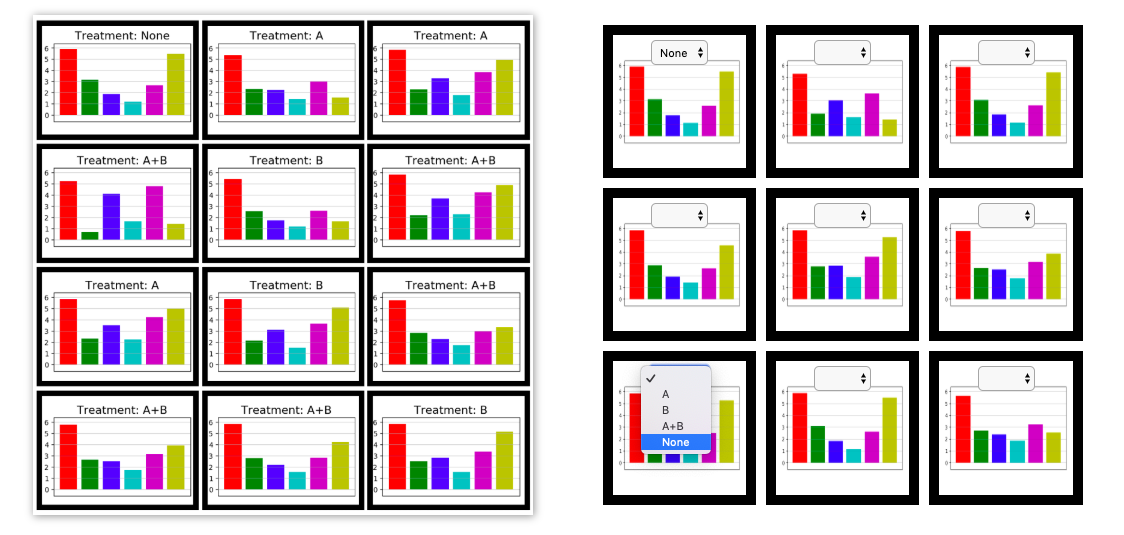
\includegraphics[width=1\columnwidth]{figures/screenshot_hiv_il.png}
\caption{The user study interface for an IL summary in the HIV simulator domain. The left side shows the summary and the right side shows the prediction states.}
\label{fig:interface_hiv_il}
\vspace{-0.2cm}
\end{figure}

\begin{figure}[H]
\centering
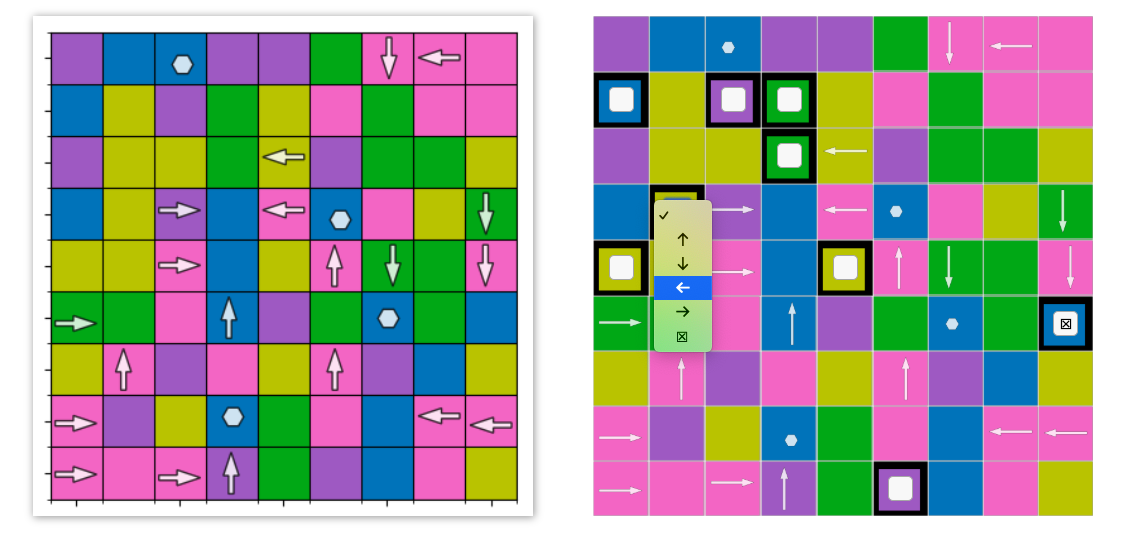
\includegraphics[width=1\columnwidth]{figures/screenshot_gridworld_il.png}
\caption{The user study interface for an IL summary in the Gridworld domain. Both sides show the full grid, the left side shows the summary and the right side shows the the prediction states (tiles surrounded by black squares with a white box inside them) as well as the actions in the summary for convenience.}
\label{fig:interface_gridworld_il}
\vspace{-0.2cm}
\end{figure}

\begin{figure}[H]
\centering
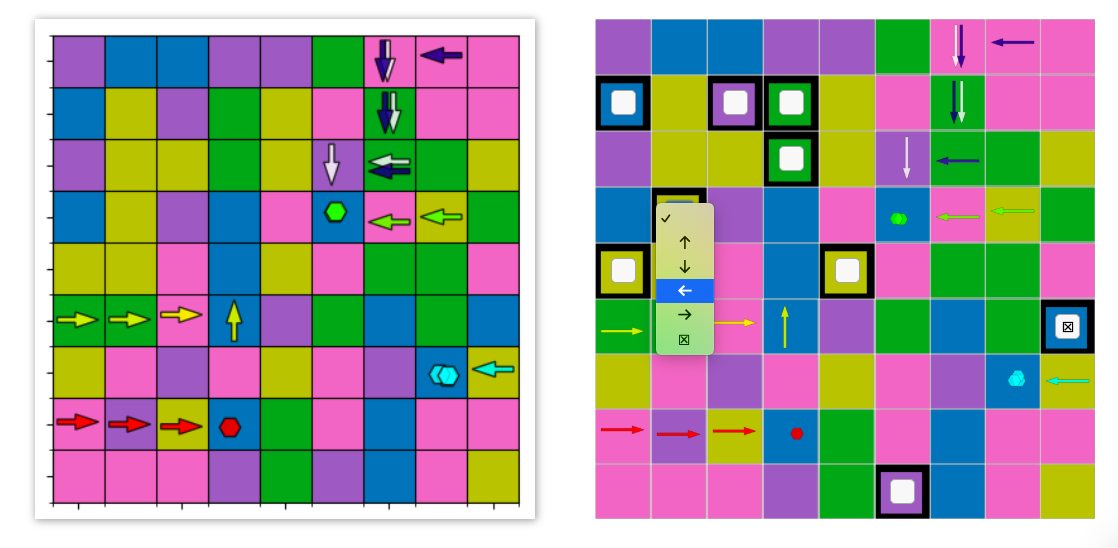
\includegraphics[width=1\columnwidth]{figures/screenshot_gridworld_irl.png}
\caption{The user study interface for an IRL summary in the Gridworld domain. Both sides show the full grid, the left side shows the summary and the right side shows the the prediction states (tiles surrounded by black squares with a white box inside them) as well as the actions in the summary for convenience. The summary displays 6 trajectories of 4 actions, corresponding to the different colored arrows.}
\label{fig:interface_gridworld_irl}
\vspace{-0.2cm}
\end{figure}

\section{Human-Subject Study Qualitative Responses}
After completing the prediction task, participants were asked to answer the following question: ``How did you decide which action the agent will take in each scenario?''. The purpose of this question was eliciting the reconstruction model people used while viewing the summary and making predictions. 

Based on the responses, we coded participants as using IL, IRL or not obviously using either. Among the IL responses we identified a few types of feature spaces to which participants referred. 

Table \ref{hiv_responses} and Table \ref{gridworld_responses} present the full set of responses for all participants in HIV simulator and Gridworld domains, respectively. These tables include the type of summary shown to the participant, the text of the response and the corresponding response type code. Table \ref{hiv_response_legend} and Table \ref{gridworld_response_legend} show the legend for the response type codes for HIV simulator and Gridworld domains, respectively. 

%HIV code legend
\begin{table}[h]
\centering
\begin{tabular}{ |c|c| }
\hline
 Code & Description \\ \hline
 IL-1 & IL - general similarity \\ 
 IL-2 & IL - absolute sizes of bars \\
 IL-3 & IL - relative bar levels \\
 IRL & IRL oriented \\
   -  & No obvious reconstruction \\
 \hline
\end{tabular}
\caption{Response types by reconstruction - HIV Simulator.
\label{hiv_response_legend}}
\end{table}

%HIV Responses
\setlength\LTleft{-1in}
\setlength\LTright{-1in}
 \begin{longtable}{ | m{0.6in} | m{5in}| m{0.6in} | }
 \caption{HIV Simulator qualitative responses encoded by response type. \label{hiv_responses}}\\
 \hline
 \multicolumn{3}{| c |}{\textbf{HIV Simulator Qualitative Responses}}\\[0.5ex]
 \hline
 \textbf{Summary} & \textbf{Response Text} & \textbf{Response Type}\\[0.5ex]
 \hline
 \endfirsthead
 
 \hline
 \textbf{Summary} & \textbf{Response Text} & \textbf{Response Type}\\[0.5ex]
 \hline
 \endhead
 
 \hline
 \endfoot
 
%  \hline
%  \multicolumn{3}{| c |}{End of Table}\\
 \hline\hline
 \endlastfoot
 
IL & I thought about the level that was displayed in the graph and then made my prediction based on the trend that I thought would follow. & IL-1 \\ \hline
IL & I tried to match the blood test to the examples. & IL-1 \\ \hline
IL & I just tried to find the graph that looked closest to the scenario and then used that to inform my decision & IL-1 \\ \hline
IL & I tried my best to find a pattern in the previous patient scenarios and use that to try to determine the treatment that the agent would choose. It was very difficult for me to find a pattern. Some of them, I just used gut instinct and went with what I thought was close to previous treatments chosen. & IL-1 \\ \hline
IL & I compared with the tests on left. & IL-1 \\ \hline
IRL & I matched it to the treatments on the left and picked the most simialr ones & IL-1 \\ \hline
IRL & I looked for a pattern in each treatment and tried to match it with the given scenario. & IL-1 \\ \hline
IL & I tried to match the blood tests that characterize the disease with the AI agent treatment. Each one had distinguishing characteristics. & IL-1 \\ \hline
IRL & Based off the patterns I saw in his previous treatments. & IL-1 \\ \hline
IRL & I mostly tried to match up the graph to the closest one in the summary, and chose the treatment it displayed. & IL-1 \\ \hline
IL & I compared the graphs of the scenarios against the treatment array I was given and chose the closest match. & IL-1 \\ \hline
IL & Tried to match to a similar patient on the left & IL-1 \\ \hline
IL & I examined the charts to see if there was one that corelated well, and then compared all of that letter to it to see if it was a common reaction. & IL-1 \\ \hline
IRL & Following the previous examples. & IL-1 \\ \hline
IL & Comparing the results to what was shown & IL-1 \\ \hline
IRL & I based it on the sequence that was presented to me. I looked at the colors of the graph and how much of each was shown and tried to match that with what I thought the agent would do next.  & IL-1 \\ \hline
IL & I tried to match up the graphs as best as I could. & IL-1 \\ \hline
IL & By assessing their blood tests and looking at prior treatments taken in similar blood tests before.  & IL-1 \\ \hline
IRL & I compared the sizes of the bars with the examples that were on the left and picked a treatment that had a similar result. & IL-1 \\ \hline
IL & I compared the images on the right with one on the left and chose the treatment based on similarity. & IL-1 \\ \hline
IRL & I tried to match them the best way I could by comparing the other scenarios.  & IL-1 \\ \hline
IL & Tried to find the closest scenario in the summary & IL-1 \\ \hline
IRL & I saw the graphs and how they looked with certain treatments and copied that & IL-1 \\ \hline
IL & I tried to find the samples that had very similar criteria for each of the blood test, including relative levels vs others as well as over all levels. & IL-1 \\ \hline
IL & Tried to find similarities in the graphs and make decisions accordingly. & IL-1 \\ \hline
IL & I chose based on the similarity of the blood tests levels from the scenarios on the left. & IL-1 \\ \hline
IL & I compared to the options given. & IL-1 \\ \hline
IRL & I compared the blood tests taken in each scenario from a previous one, and tried to replicate it. & IL-1 \\ \hline
IL & I tried to look for similarities between the completed graph and the graph that I had to fill in. If I noticed an inverse parabola, I would choose \None\ (top left). If I noticed that pink was above the tannish-yellow, I would try to correlate the degree to which it was higher and look at a similar completed graph. I tried to model my predictions of the agent's behavior based on the data that was already presented to me. & IL-1 \\ \hline
IL & I tried my best to compare the graphs & IL-1 \\ \hline
IRL & I comapred the graphs to the other graphs. & IL-1 \\ \hline
IL & I compared each set of graphs to the graphs for each treatment and tried to match similar graphs & IL-1 \\ \hline
IL & I tried to match the graphs with the treatments. For example if most of the A+B treatments seemed to form a curve on the graph I chose A+B if the graph has a curve. & IL-1 \\ \hline
IL & I tried to compare them to the similarities as shown on the left. & IL-1 \\ \hline
IRL & I looked at how similar a graph looked to one the agent treated and chose the same action that the agent chose. & IL-1 \\ \hline
IL & I tried to match the graphs with what the other had done/figure out key components of the chart. & IL-1 \\ \hline
IL & By using the examples and trying to match them accordingly. & IL-1 \\ \hline
IRL & I looked at each scenario and looked at the summary, I chose the one that I thought was similar to one that was in the summary. & IL-1 \\ \hline
IL & i looked at the same graphs & IL-1 \\ \hline
IL & I tried to match the levels with the graphs to those in the known actions, as best I could. & IL-1 \\ \hline
IRL & I compared the charts and chose the most similar treatment to the the patterns. & IL-1  \\ \hline
IRL & I was trying to look at the color graphs to compare the size & IL-2 \\ \hline
IL & Based on the values of each of the bars. & IL-2 \\ \hline
IL & I looked for patterns within the blood tests like the disparity between them. & IL-3 \\ \hline
IRL & I compared the charts and their results to the scenario I was evaluating. It seemed like there were some patterns in the bars based on the agents actions, and I tried to identify those patters as best I could. & IL-3 \\ \hline
IL & I chose the one that was closest to the levels.  & IL-3 \\ \hline
IL & I compared the size and order of the bar graphs, then guessed based on similarity. & IL-3 \\ \hline
IL & Comparative blood test tick levels & IL-3 \\ \hline
IRL & I tried to match the levels of the blood tests with another patient as much as possible and chose the same action as that one. I looked for key identifiers that separated the graph from others, such as two of the same level. & IL-3 \\ \hline
IRL & i compared the levels of each of the colors  and the shapes of the graphs.  & IL-3 \\ \hline
IRL & Relative similarity of bar heights in relationship to each-other,  inferred from previous actions.   & IL-3 \\ \hline
IRL & I tried to follow the patterns of the treatments along with the images provided and picked which was closer in relation.  & IL-4 \\ \hline
IL & Looking at past test and comparing which test were high or low and like these new tests. & IL-3 \\ \hline
IRL & I looked at the light blue/4th bar and compared how high it is to the examples. Then I looked at the dark blue bar/3rd bar, and compared also. I noticed that there were some differences in a+b or just A or B depending on how big those bars where. Plus the last bar usually indicates it's going to be a+b if its shorter. & IL-3 \\ \hline
IRL & Treatment A is used to decrease middle ones(blue, light blue and purple) and to increase light green which at the end.\n\n Treatment  is used to increase green which is second. & IRL \\ \hline
IRL & I based my answers solely on the results of each blood test. If the results were better for Treatment A, I would chose A.  & - \\ \hline
IRL & I tried to see the difference in the way the graphs moved & - \\ \hline
IL & Based on their policy & - \\ \hline
IRL & I compared it to the diagram. & - \\ \hline
IL & I just went with my intuition with what little understanding I had on how this works. & - \\ \hline
IL & this is very critical situation to find & - \\ \hline
IL & unsure what each bar represents (good or bad?), so just trying everything to see what works & - \\ \hline
IRL & The deontological class of ethical theories states that people should adhere to their obliga- tions and duties when engaged in decision making when ethics are in play. & - \\ \hline
IRL & I basically gave up & - \\ \hline
IRL & I tried to track the treatments with the bar chart & - \\ \hline
IL & if achieve in the mainly trying to reach this one. it is a treatment behavior on that ones. & - \\ \hline
IRL & Based on historical action highlighted in the bar graphs. And some luck was involved because more important data (actual numbers) was withheld.  & - \\ \hline
IL & I chose my actions based on the each patient's blood test in each scenario.  & - \\ \hline
IRL & I tried to decide based on the outcomes shown on the given charts. The most likely to be successful. & - \\ \hline
IRL & The graph results, shape and color & - \\ \hline
IRL & I tried to compare what was used. & - \\ \hline
IRL & what seemed best & - \\ \hline

 \end{longtable}

%Gridworld code legend
\begin{table}[h]
\centering
\begin{tabular}{ |c|c| }
\hline
 Code & Description \\ \hline
 IL-1 & IL - actions in similar tiles \\ 
 IL-2 & IL - direction \\
 IL-3 & IL - frequent action for color \\
 IL-4 & IL - surrounding tiles \\
 IRL  & IRL - goal oriented \\
   -  & No obvious reconstruction \\
 \hline
\end{tabular}
\caption{Response types by reconstruction - Gridworld.
\label{gridworld_response_legend}}
\end{table}

%Gridworld responses
\setlength\LTleft{-1in}
\setlength\LTright{-1in}
 \begin{longtable}{ | m{0.6in} | m{5in}| m{0.6in} | }
 \caption{Gridworld qualitative responses encoded by response type. \label{gridworld_responses}}\\
 
 \hline
 \multicolumn{3}{| c |}{\textbf{Gridworld Qualitative Responses}}\\[0.5ex]
 \hline
 \textbf{Summary} & \textbf{Response Text} & \textbf{Response Type}\\[0.5ex]
 \hline
 \endfirsthead
 
 \hline
 \textbf{Summary} & \textbf{Response Text} & \textbf{Response Type}\\[0.5ex]
 \hline
 \endhead
 
 \hline
 \endfoot
 
%  \hline
%  \multicolumn{3}{| c |}{End of Table}\\
 \hline\hline
 \endlastfoot
 
IL & I thought they would act similarly to other tiles of the same color. & IL-1 \\ \hline
IL & I looked at what action was being taken in similar colored blocks and used that information to help me make my judgments. & IL-1 \\ \hline
IRL & based on actions took in tiles of the same color & IL-1 \\ \hline
IRL & I looked at what each color arrow did in each colored tile. & IL-1 \\ \hline
IRL & I tried to follow what I felt the directional pattern was. & IL-2 \\ \hline
IL & I tried to see what direction most of the arrows where taking and tried to see if it would be appropriate to follow the same position as the arrows already shown.  & IL-2 \\ \hline
IL & I looked at all the arrows and most of them in the same columns were going the same direction, so that's what I chose & IL-2 \\ \hline
IL & I tried comparing the colors and deciding which was more frequent for a color.  & IL-3 \\ \hline
IL & I tried to guess based on the colors and directions that seemed to be favored in the arrows displayed on the summary. & IL-3 \\ \hline
IRL & I was trying to be consistent with what colors had what action on it. & IL-3 \\ \hline
IL & I tried to use the nearest tile as a guide. & IL-4 \\ \hline
IL & I decided by the surrounding arrows If most were up I would click on the up arrow & IL-4 \\ \hline
IL & By looking at the summery and seeing which way the marked tiles were moving around the marked tile i thought it was more likely to follow the same pattern. & IL-4 \\ \hline
IL & I looked at the surrounding block and went with the most common move. If there was a surrounding block that was also the same color then that took priority. & IL-4 \\ \hline
IL & I tried looking to see where the majority of the arrows were going to, and chose those to move to, which seemed to be blue and green. & IRL \\ \hline
IL & I figured each section would have a beginning and lead to a stop square, so I marked the square accordingly.  & IRL \\ \hline
IL & I was trying to make the fastest path to a blue square & IRL \\ \hline
IL & It seems like the agent tries to get to blue in as few moves as possible, and then stops there. I chose based on that reasoning. & IRL \\ \hline
IL & I chose the one that I thought would get them to the higher point squares or blue. & IRL \\ \hline
IL & I tried to get it to go to a blue spot, because I think that's what it wanted & IRL \\ \hline
IL & The first time I was just attempting to do something similar to the given board, however, the second time I ranked the colors.  & IRL \\ \hline
IRL & Which would take them to where there was a stop & IRL \\ \hline
IRL & I tried to predict how they could end up at the stops in place. & IRL \\ \hline
IRL & The agent seems to prefer to stop on blue squares, so I chose actions that led to blue squares. & IRL \\ \hline
IRL & I generally assumed it would take the shortest path to a blue square and guessed accordingly. & IRL \\ \hline
IRL & I pushed them in the shortest direction to a blue square, or stopped if they were already on one. & IRL \\ \hline
IRL & I decided that the computer seems to be always working towards a blue square. I chose the simplest path to get to a blue square.  & IRL \\ \hline
IL & The agent seems primarily motivated to getting to the blue squares and stopping. So I selected directions that would move the agent toward the blue squares. & IRL \\ \hline
IRL & The agent chooses the shortest path to the nearest blue square. & IRL \\ \hline
IRL & I figured that the agent was attempting to get to (and stay on) the blue squares, so I assumed the agent would take the fewest steps possible to reach a blue square. I assumed it would take the action that would get it closest to a blue square. & IRL \\ \hline
IRL & I think blue is always stop. It seems the agent travels to a stop. There may be a task to perform at that spot. & IRL \\ \hline
IRL & I tried to make a path according to the other arrows. I figured they run a few squares before they stop. Seemed they stopped in blue square so made one a stop in the blue square. & IRL \\ \hline
IRL & I decided that the agent would take the shortest route available to the nearest blue tile.  & IRL \\ \hline
IRL & I thought the agent was trying to go to the nearest blue square and stop there. It seemed to prefer to go sideways but I could not decide if it preferred to go left or right or toward the center of the diagram. & IRL \\ \hline
IL & I decided which action the agent would take based on the amount of room that they had, which way the other agents were going, and how they could get the most points. & - \\ \hline
IL & Honestly, just guessing. & - \\ \hline
IL & I honestly have no idea, except that I followed the behavior of the closest tile with a behavior either in a column or in a row. & - \\ \hline
IL & I looked at the arrows already there as well as the stops and tried to ascertain the clearer path. & - \\ \hline
IL & To be honest I guessed in an intuitive manner, I can not really explain it. & - \\ \hline
IL & If there was a color tile that matched in a way that it could move. & - \\ \hline
IL & I just looked at where the arrows were headed and guessed the direction he wanted to go. I made sure not to overlap existing moves. & - \\ \hline
IL & I completely guessed. & - \\ \hline
IL & Just kind of guessed I guess. Didn't want them to cross any paths or back track. & - \\ \hline
IL & I looked at the surrounding movements and saw what would make sense for it to get there. & - \\ \hline
IL & I went with what appeared to be the most logical steps and also took into account what the board was displaying & - \\ \hline
IL & I guess it was just a gut feeling and trying to find patterns. & - \\ \hline
IRL & Some arrows and directions matched up to a sequence. Others, were a guess. & - \\ \hline
IRL & I observed the agents steps taken in the last scenario. & - \\ \hline
IRL & I tried to see where the arrows were going to and to follow a similar pattern. & - \\ \hline
IRL & I tried to visualize how the agent maybe would naturally be moving. & - \\ \hline
IRL & i predicted the action s that will be taken by the agent in the maptiles & - \\ \hline
IRL & tried to see the sequence & - \\ \hline
IRL & I looked at the directions he already traveled in the color I was judging and tried to think about where it might go next. & - \\ \hline
IL & I tried to intuit which decision would be the most effective & - \\ \hline
IL & I tried to imagine what the most logical move would be for the agent. & - \\ \hline
IL & I looked at what they did in the squares around it & - \\ \hline
IL & I looked at the arrows around the boxes & - \\ \hline
IL & I looked at the surrounding colors and details of the arrows/stops and chose around that & - \\ \hline
IL & I looked at the color of the squares they mostly preferred to move toward, then decided how they would act based on that. & - \\ \hline
IRL & I made a guess based on the actions in the surrounding squares. & - \\ \hline
IRL & guessed & - \\ \hline
IRL & I went with what the agent had done the precious 3 turns & - \\ \hline
IRL & I tried to use the image on the left for guidance but ultimately went with what made since, based on the position of the white square. & - \\ \hline
IRL & I just made my choices by what would make sense on the grid & - \\ \hline
IRL & I followed the sequebce of the arrow. & - \\ \hline
IRL & It seems a reasonable way to go based on the potential movements.  & - \\ \hline
IRL & I just tried to think what would be most logical. & - \\ \hline
IRL & It seem like the best case scenario with a little guess work thrown in. & - \\ \hline
IRL & i thought about the way that made the most sense and choice that & - \\ \hline
IRL & I looked at the other summaries and tried to find a pattern and based it on that & - \\ \hline
IRL & look at what it did before when faced with options it faces now based on color available in the legal moves & - \\ \hline
IRL & I looked at the tiles to see what he mostly was navigating towards, in favor over another choice. & - \\ \hline
IRL & I tried to predict the next movement as closely as I could. If it seemed likely, then I decided on that specific action. & - \\ \hline
IRL & I think I just went with following the general consensus of where the other agents nearby seemed to be headed. & - \\ \hline
IRL & Just a gut feeling honestly. & - \\ \hline
 
\end{longtable}




\end{document}